\documentclass{fizykalab}

% Ustawienia do tabelki

\wydzial{WI}
\autorjeden{Piotr Karamon}
\autordwa{Hubert Kasprzycki}
\rok{2}
\grupa{12}
\zespol{5}
\temat{Efekt fotoelektryczny}
\nrcwiczenia{82}
\datawykonania{31.10.2023}
\dataoddaniajeden{07.11.2023}
\zwrotdopoprawy{}
\dataoddaniadwa{}
\datazaliczenia{}

\usepackage{amsmath}
\usepackage{amsfonts}
\usepackage{parskip}
\usepackage{multirow}

\newenvironment{conditions}[1][gdzie:]
  {#1 \begin{tabular}[t]{>{$}l<{$} @{${} - {}$} l}}
  {\end{tabular}\\[\belowdisplayskip]}

% \renewcommand{\arraystretch}{1.5}
\newcolumntype{L}[1]{>{\raggedright\let\newline\\\arraybackslash\hspace{0pt}}m{#1}}
\newcolumntype{C}[1]{>{\centering\let\newline\\\arraybackslash\hspace{0pt}}m{#1}}
\newcolumntype{R}[1]{>{\raggedleft\let\newline\\\arraybackslash\hspace{0pt}}m{#1}}

\usepackage[left=1.75cm, right=2cm, top=3cm]{geometry}
\usepackage[labelfont=bf]{caption}

\newcommand{\nm}{\ensuremath{\text{nm}}}
\newcommand{\mm}{\ensuremath{\text{mm}}}
\newcommand{\m}{\ensuremath{\text{m}}}
\newcommand{\vthz}{\ensuremath{\frac{\text{V}}{\text{THz}}}}
\newcommand{\volt}{\ensuremath{\text{V}}}
\newcommand{\Js}{\ensuremath{\text{Js}}}
\newcommand{\echarge}{\ensuremath{1.602 \cdot 10^{-19} \text{C}}}


\usepackage{natbib}
\usepackage{url}
\begin{filecontents*}{test.bib}
@MISC{elportal-zlacze,
    author = {Michał Kurzela},
    title = {Dioda prostownicza - charakterystyka, oznaczenia, budowa},
    year = {2022},
    note = {[\url{https://elportal.pl/i/2022/09/06/12517-cfe4-1600x0_089-04.jpg}; odwiedzona  14.10.2023]},
    url = {https://elportal.pl/i/2022/09/06/12517-cfe4-1600x0_089-04.jpg}
}
\end{filecontents*}

\begin{document}

\maketitle

\section{Cel ćwiczenia}
Badanie zależności energii fotoelektronów w zależności od długości światła padającego na
metal. Wyznaczanie stałej Plancka i pracy wyjścia.

\section{Wstęp teoretyczny}
Światło ma naturę dualną – korpuskularno-falową. 
Możliwe do zaobserwowania zjawisko fotoelektryczne
zewnętrzne polegające na emisji elektronów z powierzchni metalu dowodzi jego właściwościom korpuskularnym.
Emisja elektronów nie zależy od
intensywności, lecz od częstotliwości światła. 
Istnieje graniczna częstotliwości,
poniżej której nie obserwuje się tego zjawiska.
Energia kinetyczna emitowanych elektronów jest ograniczona pewną wartością
jako $E_{\text{kmax}}$ i wartość
ta zależy wyłącznie od częstotliwości fali i użytego metalu.
Energia kinetyczna emitowanych
elektronów zawiera się w przedziale $[0, E_{\text{kmax}}]$ i nie obserwuje się elektronów o wyższej energii.

Energię fotonu można wyliczyć ze wzoru:

\begin{equation}
    E_{v} = hv = \frac{hc}{\lambda}
\end{equation}

\begin{conditions}
    h & stała Plancka \\
    v & częstotliwość padającej fali \\
    c & prędkość światła \\
    \lambda & długość fali padającego światła
\end{conditions}

Maksymalna energia kinetyczna elektronu wyraża się wzorem

\begin{equation}
    E_{\text{kmax}} = E_v - W 
\end{equation}

\begin{conditions}
    W & praca wyjścia
\end{conditions}

Maksymalną energię kinetyczną $E_\text{kmax}$ można
zmierzyć dobierając takie napięcie zewnętrzne,
że mierzony prąd zmaleje do 
0. W takiej sytuacji $eU_h$ równe jest $E_{kmax}$.

\begin{equation}
    \label{eq:uh}
    U_h = \frac{h}{e} v - \frac{W}{e}
\end{equation}


\section{Aparatura pomiarowa}

\begin{figure}[H]
    \centering
    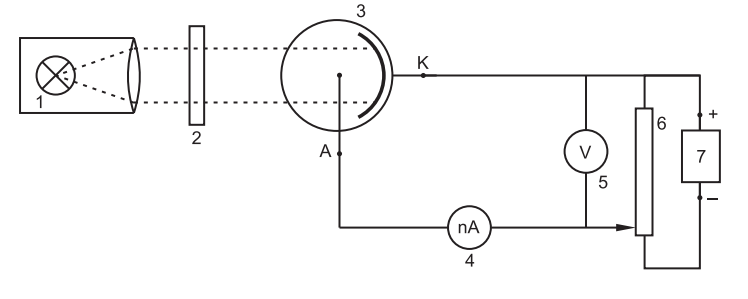
\includegraphics[width=0.75\linewidth]{aparatura.png}
    \caption{Schemat aparatury do wyznaczania stałej Plancka}
\end{figure}

\begin{enumerate}
    \item żarówka
    \item filtry barwne
    \item fotokomórka, A – anoda, K – katoda
    \item nanoamperomierz
    \item woltomierz
    \item potencjometr
    \item stabilizowany zasilacz napięcia stałego 
\end{enumerate}

\section{Przebieg doświadczenia}
Na początku uruchomiliśmy układ pomiarowy. Dla każdego filtra barwnego 
trzykrotnie zmierzyliśmy wartość 
natężenia prądu dla napięcia $U_\text{a-f} = 0$,
oraz wartość napięcia odcięcia $U_h$, dla którego natężenie
prądu było równe 0.
Wyniki przedstawiliśmy w tabeli 1.
Następnie znając zakres prądu pomiędzy $I = 0$ 
a wartością $I$ dla $U_\text{a-f} = 0$,
podzieliśmy go na około 10 przedziałów i zmierzyliśmy zależność prądu 
fotokomórki od napięcia hamującego. Dane zebraliśmy w tabeli 2.

\section{Wyniki pomiarów}

\begin{table}[H]
\centering
\caption{Wyniki pomiarów zależności napięcia hamowania $U_h$ od częstotliwości $v$}
\begin{tabular}{|l|l|l|l|c|}
\hline
    \textbf{\begin{tabular}[c]{@{}l@{}}Kolor/ \\ długość fali [nm] \end{tabular}} &
    \begin{tabular}[c]{@{}l@{}}Częstotliwość \\ $v=c/\lambda$ {[}Hz{]} \end{tabular} & 
    \begin{tabular}[c]{@{}l@{}} $I$ {[}uA{]} \\ (dla $U_\text{a-f}=0$) \end{tabular} & 
    \begin{tabular}[c]{@{}l@{}} $U_h$ [V] \\ (dla I=0) \end{tabular} & 
    $U_\text{$h,\text{śred.}$}$ {[}V{]} \\ \hline
\multirow{3}{*}{\textbf{Zielony / 500}}   & \multirow{3}{*}{599,585}  & 2,23 & 0,45  & \multirow{3}{*}{0,449}       \\ \cline{3-4}
                                             & & 2,21 & 0,449 &                              \\ \cline{3-4}
                                             & & 2,2  & 0,448 &                              \\ \hline
\multirow{3}{*}{\textbf{Żółty / 590}}        & \multirow{3}{*}{508,123} & 3,37 & 0,392 & \multirow{3}{*}{0,3903} \\ \cline{3-4}
                                             &  & 3,3  & 0,39  &                              \\ \cline{3-4}
                                             &  & 3,28 & 0,389 &                              \\ \hline
\multirow{3}{*}{\textbf{Fioletowy / 480}} & \multirow{3}{*}{624,568}  & 2,41                & 0,565               & \multirow{3}{*}{0,5653}                     \\ \cline{3-4}
                                             &  & 2,42 & 0,566 &                              \\ \cline{3-4}
                                             &  & 2,43 & 0,565 &                              \\ \hline
\multirow{3}{*}{\textbf{Czerwony / 630}} & \multirow{3}{*}{475,861} & 0,34 & 0,26  & \multirow{3}{*}{0,258}       \\ \cline{3-4}
                                             &  & 0,33 & 0,258 &                              \\ \cline{3-4}
                                             &  & 0,33 & 0,256 &                              \\ \hline
\end{tabular}
\end{table}


\begin{table}[H]
\centering
\caption{Zależność prądu fotokomórki I od napięcia hamującego $U_\text{a-f}$}
\begin{tabular}{|l|l|l|l|l|l|l|l|l|l|l|l|}
\hline
  \textbf{\begin{tabular}[c]{@{}l@{}} \text{kolor 1}/\\ dł.fali \\ {[}nm{]} \end{tabular}} &
  $I$ {[}uA{]} &
  $U_\text{a-f}$ {[}V{]} &
  \textbf{\begin{tabular}[c]{@{}l@{}} \text{kolor 2}/\\ dł.fali \\ {[}nm{]} \end{tabular}} &
  $I$ {[}uA{]} &
  $U_\text{a-f}$ {[}V{]} &
  \textbf{\begin{tabular}[c]{@{}l@{}} \text{kolor 3}/\\ dł.fali \\ {[}nm{]} \end{tabular}} &
  $I$ {[}uA{]} &
  $U_\text{a-f}$ {[}V{]} &
  \textbf{\begin{tabular}[c]{@{}l@{}} \text{kolor 4}/\\ dł.fali \\ {[}nm{]} \end{tabular}} &
  $I$ {[}uA{]} &
  $U_\text{a-f}$ {[}V{]} \\ \hline
\multirow{14}{*}{\begin{tabular}[c]{@{}l@{}}Zielony\\ 500\end{tabular}} &
  0 &
  0,447 &
  \multirow{14}{*}{\begin{tabular}[c]{@{}l@{}}Żółty\\ 590\end{tabular}} &
  0 &
  0,388 &
  \multirow{14}{*}{\begin{tabular}[c]{@{}l@{}}Fioletowy\\ 480\end{tabular}} &
  0 &
  0,565 &
  \multirow{14}{*}{\begin{tabular}[c]{@{}l@{}}Czerwony\\ 630\end{tabular}} &
  0 &
  0,27 \\ \cline{2-3} \cline{5-6} \cline{8-9} \cline{11-12} 
 & 0,2 & 0,366 &  & 0,3 & 0,328 &  & 0,2  & 0,47  &  & 0,03 & 0,232 \\ \cline{2-3} \cline{5-6} \cline{8-9} \cline{11-12} 
 & 0,4 & 0,309 &  & 0,6 & 0,281 &  & 0,4  & 0,395 &  & 0,06 & 0,195 \\ \cline{2-3} \cline{5-6} \cline{8-9} \cline{11-12} 
 & 0,6 & 0,263 &  & 0,9 & 0,238 &  & 0,6  & 0,336 &  & 0,09 & 0,172 \\ \cline{2-3} \cline{5-6} \cline{8-9} \cline{11-12} 
 & 0,8 & 0,222 &  & 1,2 & 0,201 &  & 0,8  & 0,286 &  & 0,12 & 0,144 \\ \cline{2-3} \cline{5-6} \cline{8-9} \cline{11-12} 
 & 1   & 0,184 &  & 1,5 & 0,165 &  & 1    & 0,243 &  & 0,15 & 0,122 \\ \cline{2-3} \cline{5-6} \cline{8-9} \cline{11-12} 
 & 1,2 & 0,149 &  & 1,8 & 0,134 &  & 1,2  & 0,202 &  & 0,18 & 0,099 \\ \cline{2-3} \cline{5-6} \cline{8-9} \cline{11-12} 
 & 1,4 & 0,117 &  & 2,1 & 0,103 &  & 1,4  & 0,165 &  & 0,21 & 0,075 \\ \cline{2-3} \cline{5-6} \cline{8-9} \cline{11-12} 
 & 1,6 & 0,085 &  & 2,4 & 0,074 &  & 1,6  & 0,129 &  & 0,24 & 0,057 \\ \cline{2-3} \cline{5-6} \cline{8-9} \cline{11-12} 
 & 1,8 & 0,054 &  & 2,7 & 0,046 &  & 1,8  & 0,096 &  & 0,27 & 0,036 \\ \cline{2-3} \cline{5-6} \cline{8-9} \cline{11-12} 
 & 2   & 0,027 &  & 3   & 0,018 &  & 2    & 0,063 &  & 0,3  & 0,019 \\ \cline{2-3} \cline{5-6} \cline{8-9} \cline{11-12} 
 & 2,2 & 0     &  & 3,2 & 0     &  & 2,2  & 0,033 &  & 0,33 & 0     \\ \cline{2-3} \cline{5-6} \cline{8-9} \cline{11-12} 
 &     &       &  &     &       &  & 2,4  & 0,002 &  &      &       \\ \cline{2-3} \cline{5-6} \cline{8-9} \cline{11-12} 
 &     &       &  &     &       &  & 2,42 & 0     &  &      &       \\ \hline
\end{tabular}
\end{table}

\section{Opracowanie wyników}

Na podstawie danych z tabeli 1 stworzyliśmy wykres,
oraz dopasowaliśmy do niego prostą.
\begin{figure}[H]
    \centering
    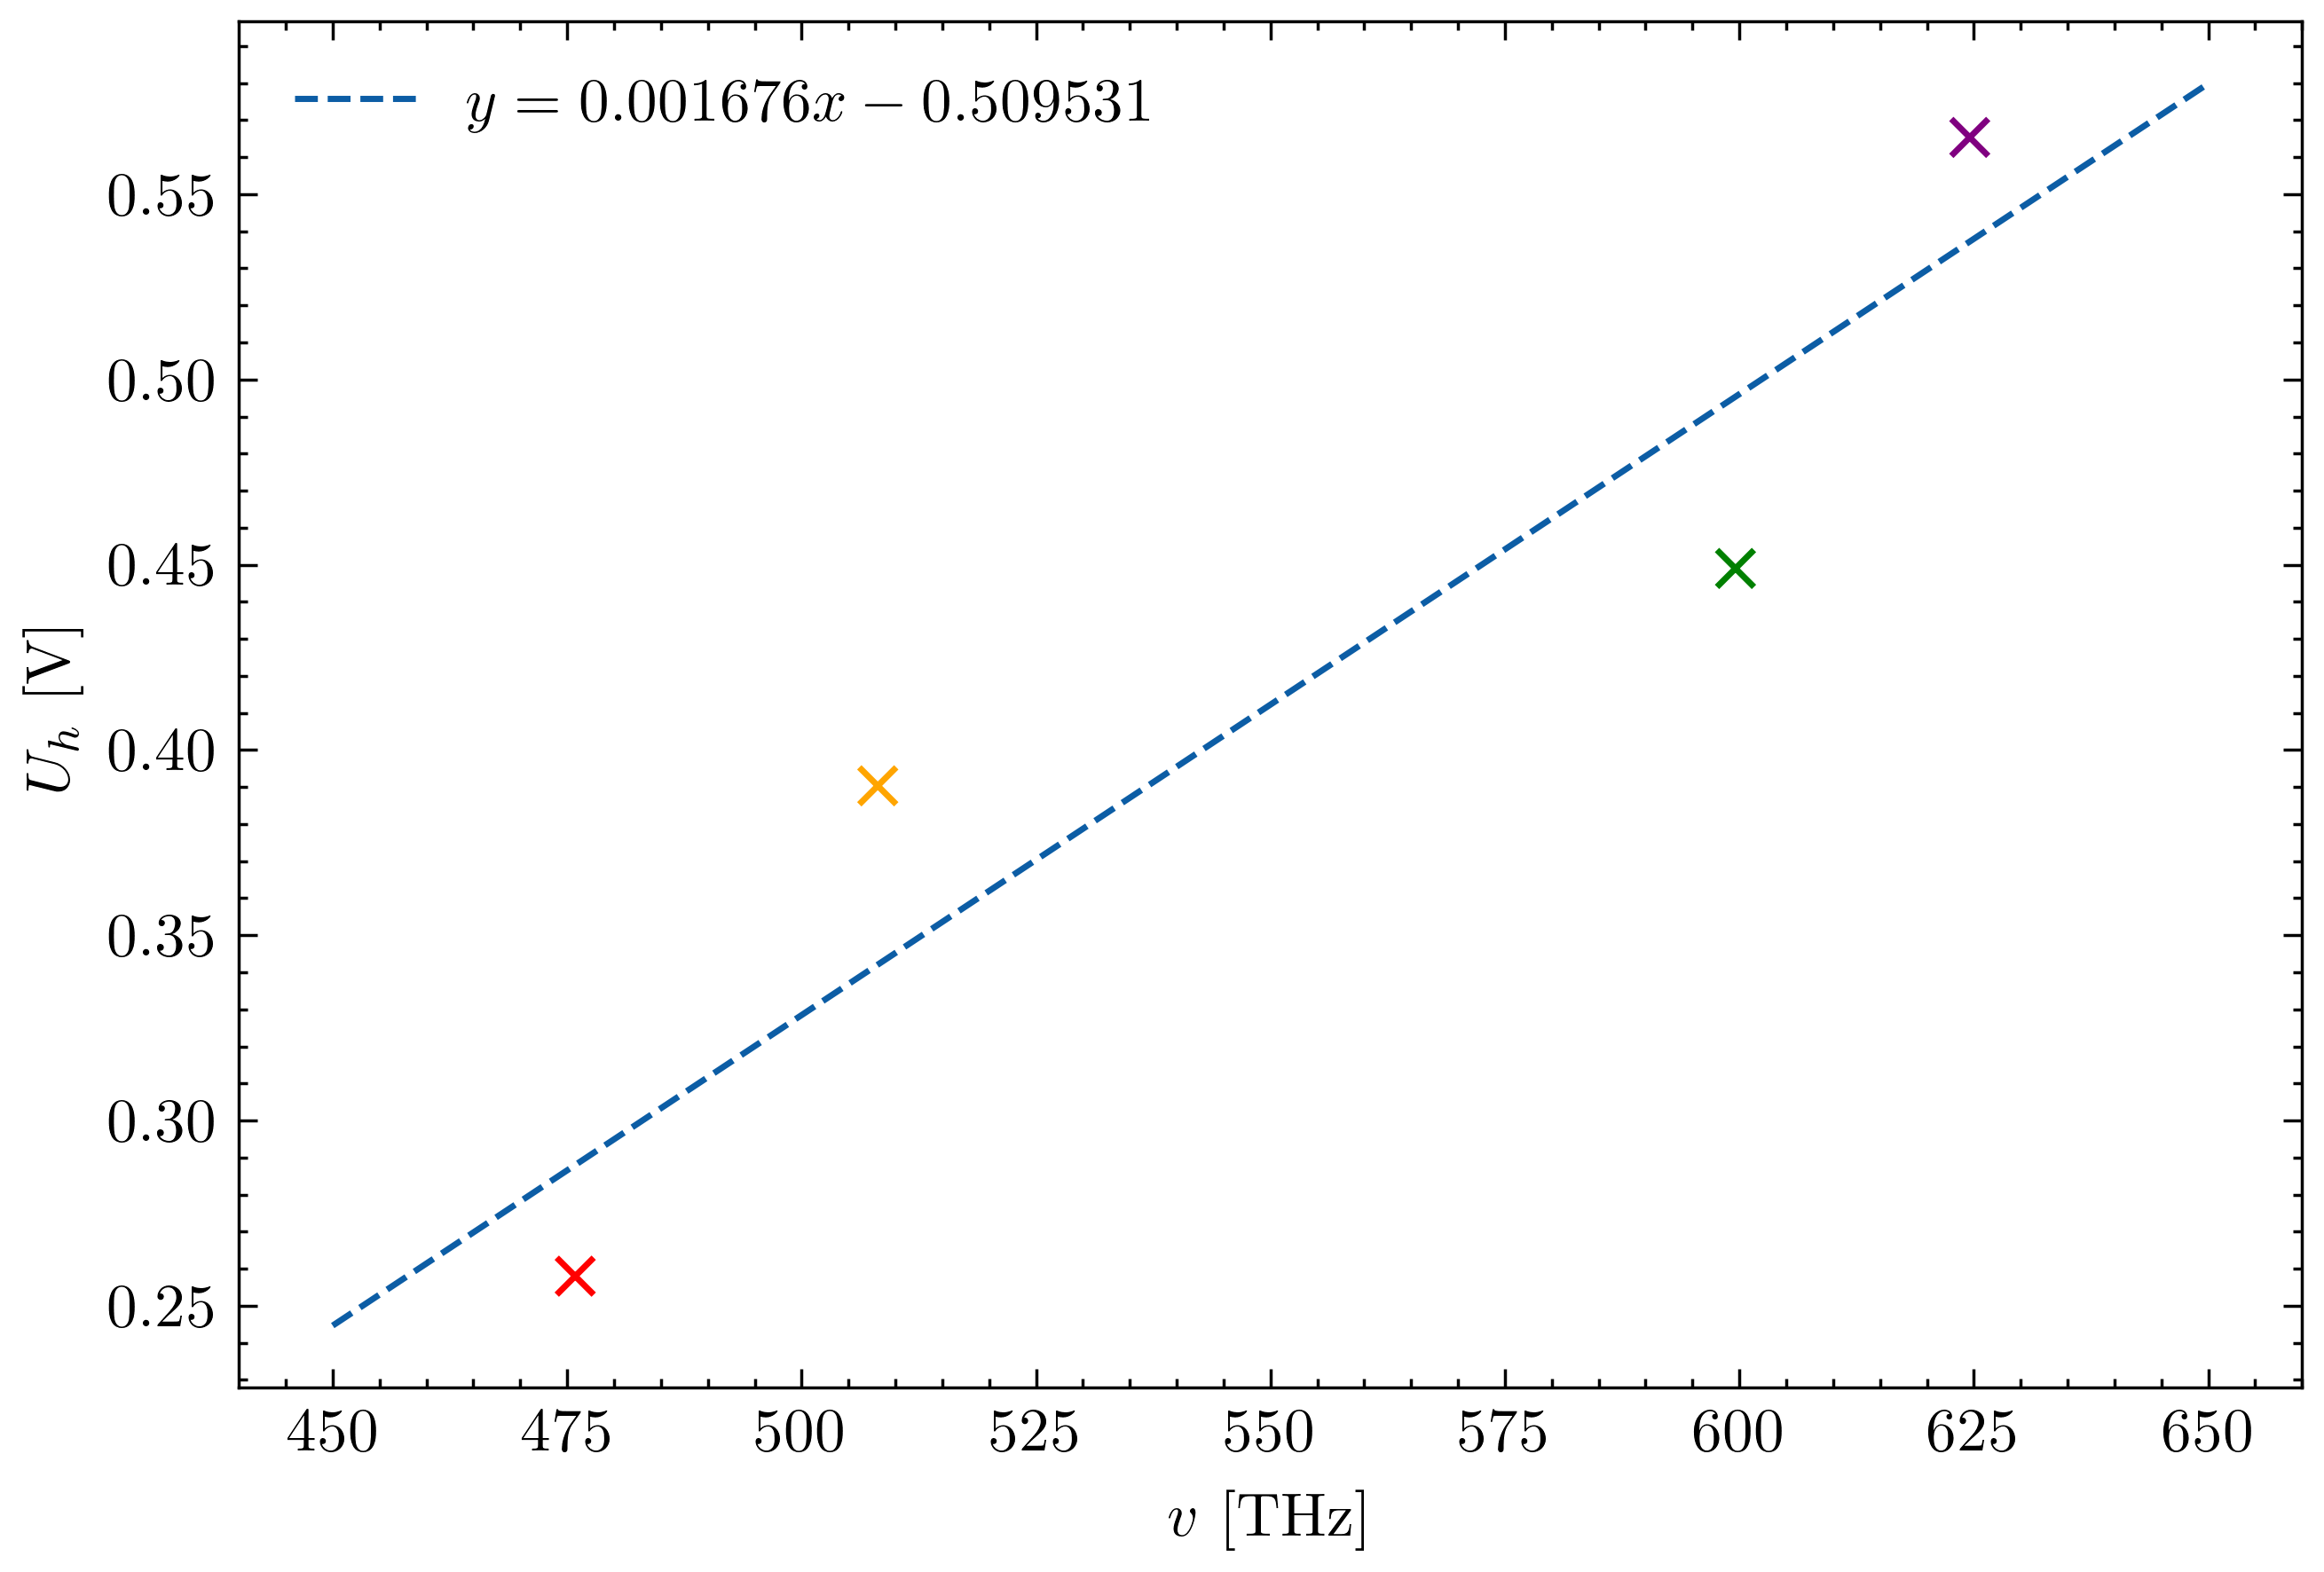
\includegraphics[width=0.75\linewidth]{allColorsFreq.png}
    \caption{Wykres zależności napięcia hamowania od częstotliwości fal poszczególnych kolorów 
    wraz z dopasowaną prostą do wykresu.
    W teorii punkty pomiarowe
    powinny znajdować się blisko dopasowanej krzywej,
    tak jednak nie jest i widać wyraźnie duże
    odległości pomiędzy punktami pomiarowymi a prostą. }
\end{figure}

Dopasowana prosta ma równanie
\begin{equation*}
    y = 0.001676x - 0.509531
\end{equation*}

Niepewności współczynników prostej są równe:
\begin{equation*}
    u(a) = 0.00045 \vthz, \quad u(b) = 0.25 \volt
\end{equation*}

Z równania (\ref{eq:uh}) wynika, że
\begin{align*}
    a &= \frac{h}{e}\\
    b &=  -\frac{W}{e}
\end{align*}

a zatem z powyższych równań możemy wyznaczyć stałą
Plancka $h$ oraz pracę wyjścia $W$

\begin{align*}
    h &= a \cdot e = 0.001676 \vthz \cdot \echarge
    = 2.68 \cdot 10^{-34} \Js \\
    W &=  -b \cdot e = 0.509531 \volt
    \cdot \echarge  = 0.510 \text{eV}
\end{align*}

W celu obliczenia niepewności pomiaru $h$ oraz $W$
wykorzystujemy prawo przenoszenia niepewności, zatem
\begin{align*}
    u(h) &= \sqrt{ \left( \frac{\partial h}{\partial a} u(a) \right)^2}  
    = \left|e \cdot u(a) \right| = \echarge \cdot 0.00045 \vthz =
    0.72 \cdot 10^{-34} \Js \\
    u(W) &= \sqrt{ \left( \frac{\partial W}{\partial b} u(b) \right)^2}  
    = \left|-e \cdot u(b) \right| = 
    \echarge \cdot 0.25 \volt = 0.25 \text{eV}
\end{align*}

Podsumowując:
\begin{align*}
    h &= 2.68 \cdot 10^{-34} \Js; \quad    u(h)  = 0.72 \cdot 10^{-34} \Js \\
    W &= 0.51 \volt; \quad u(W)  = 0.25 \volt
\end{align*}

Niepewność rozszerzona $U(h)$ jest równa
$U(h) = 2 u(h) = 1.44 \cdot 10^{-34} \Js$
,a zatem wyliczona przez nas wartość stałej 
Plancka nie jest zgodna z wartością tablicową
równą $h_\text{tab} = 6.63 \cdot 10^{-34} \Js$.
Wyliczona przez nas wartość stałej Plancka jest wyraźnie
zaniżona, a jej niepewność jest bardzo duża.

Tak duża niepewność i tak duże odchylenie od wartość 
tabelarycznej wynika najpewniej z:
\begin{itemize}
    \item Wad instrumentów pomiarowych.
    \item Faktu, że mierzymy wartości bardzo małe i
    podczas pomiarów nawet niewielkie
    zakłócenia i zaburzenia w otoczeniu 
    mogą mieć znaczący wpływ na 
    wyniki.
    \item Długości fali zostały nam podane z
    dokładnością do $0.01 \mu \text{A}$,
    nie mogliśmy sprawdzić poprawności 
    tych wartości, więc założyliśmy, że są
    słuszne, być może tak nie było.
    \item Błędy i niedokładności ludzkie.



    
\end{itemize}

Niepewność pracy wyjścia jest 
ogromna. Niepewność względna 
czyli $\frac{u(W)}{W}$ równa się, aż $49\%$.

W doświadczeniu badaliśmy zależność prądu 
fotokomórki $I$ od napięcia hamującego, 
wynikiem tego są następujące wykresy:





\begin{figure}[H]
    \centering
    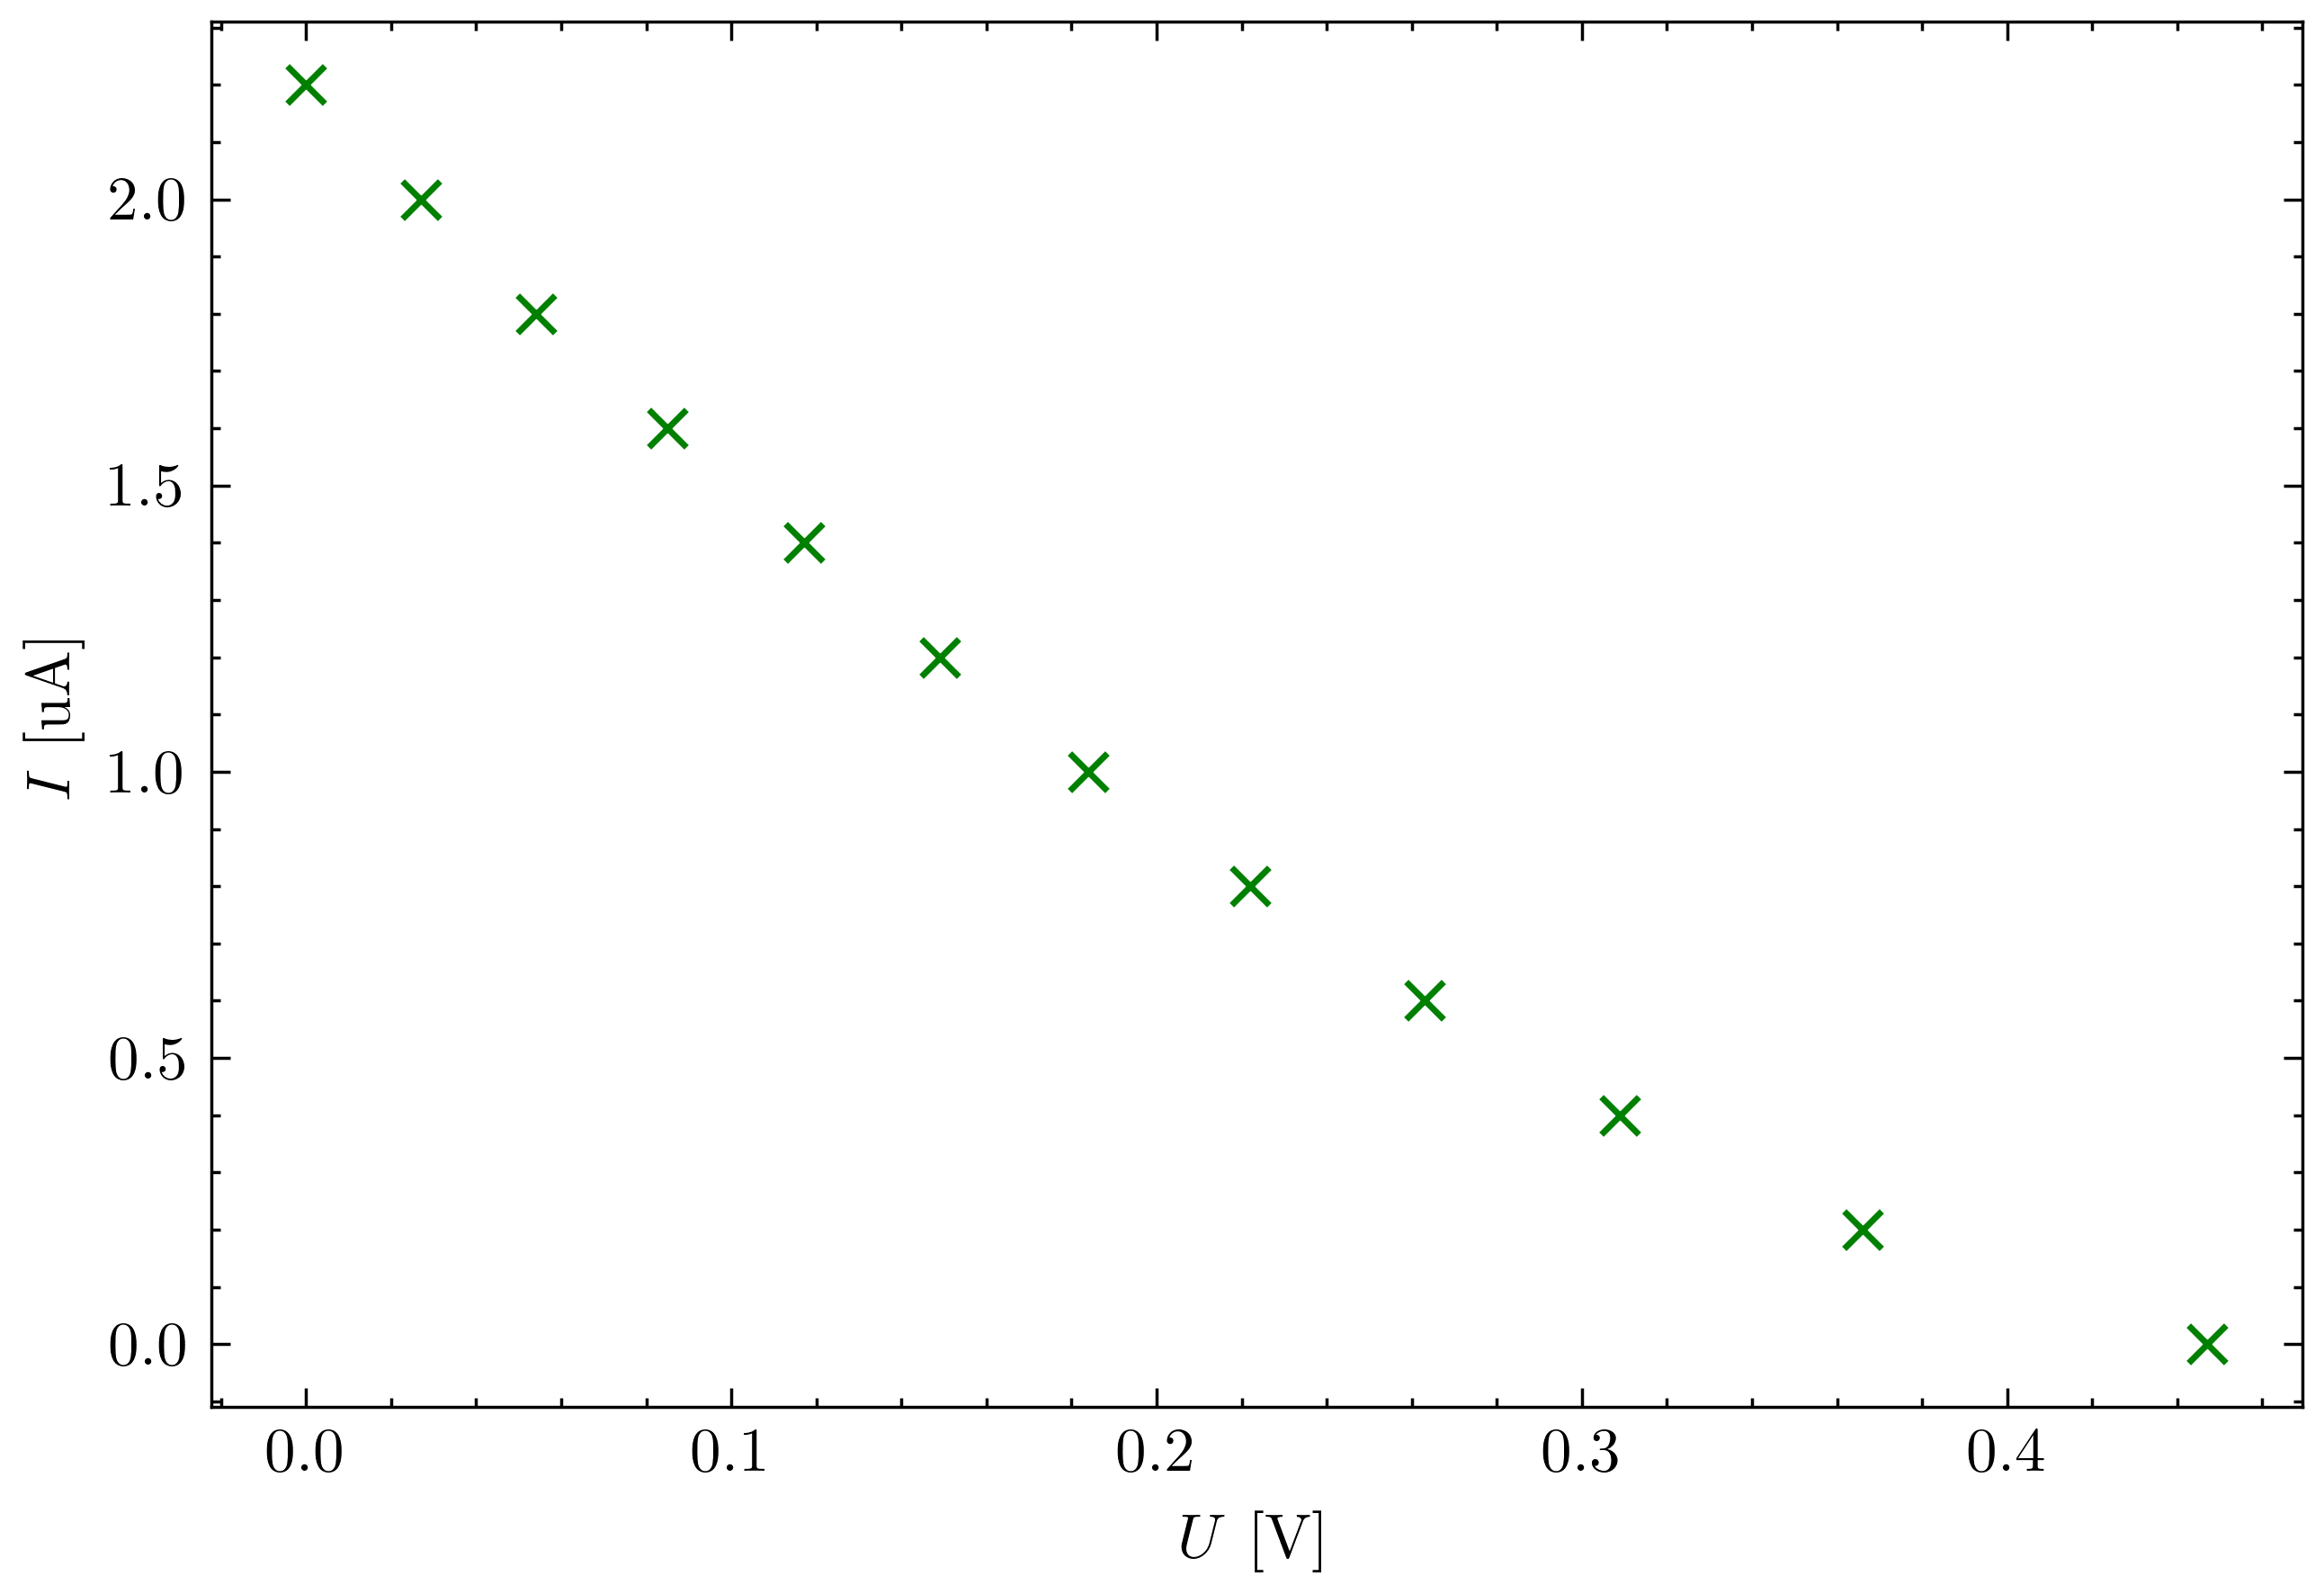
\includegraphics[width=0.75\linewidth]{green.png}
    \caption{
    Zależność prądu fotokomórki $I$ od napięcia hamującego $U$
    dla koloru zielonego.}
\end{figure}

\begin{figure}[H]
    \centering
    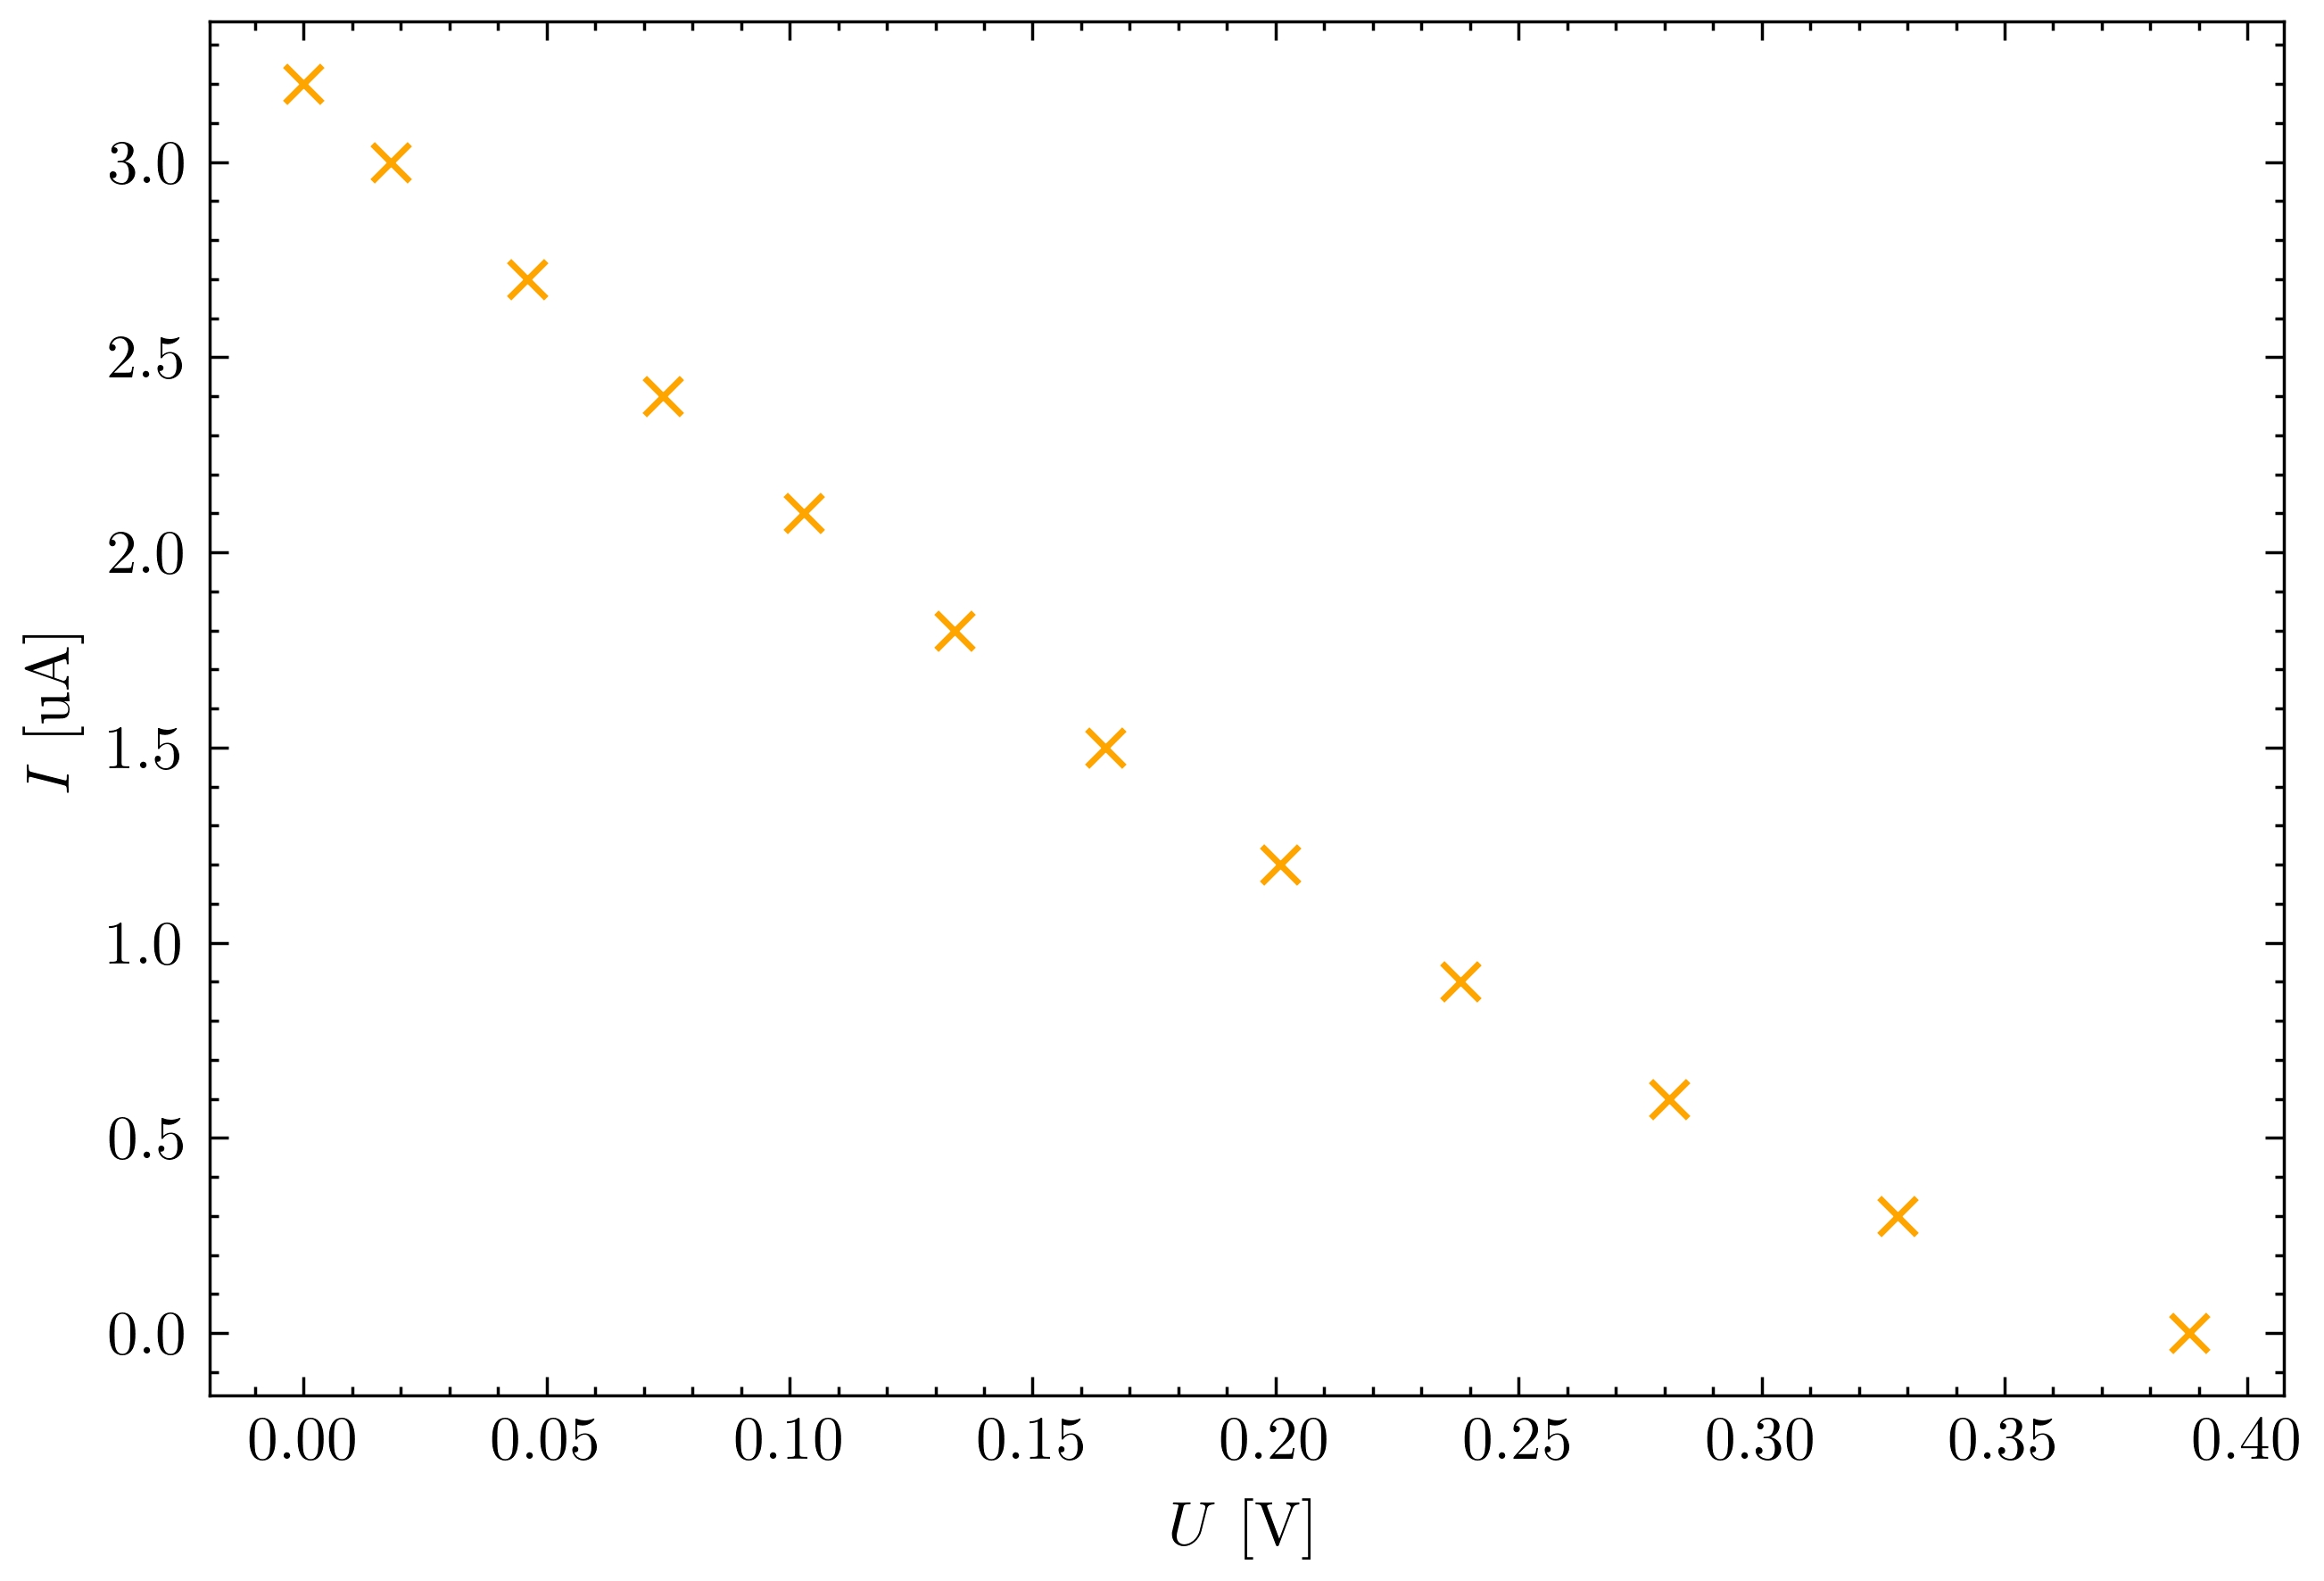
\includegraphics[width=0.75\linewidth]{yellow.png}
    \caption{
    Zależność prądu fotokomórki $I$ od napięcia hamującego $U$
    dla koloru żółtego.}
\end{figure}

\begin{figure}[H]
    \centering
    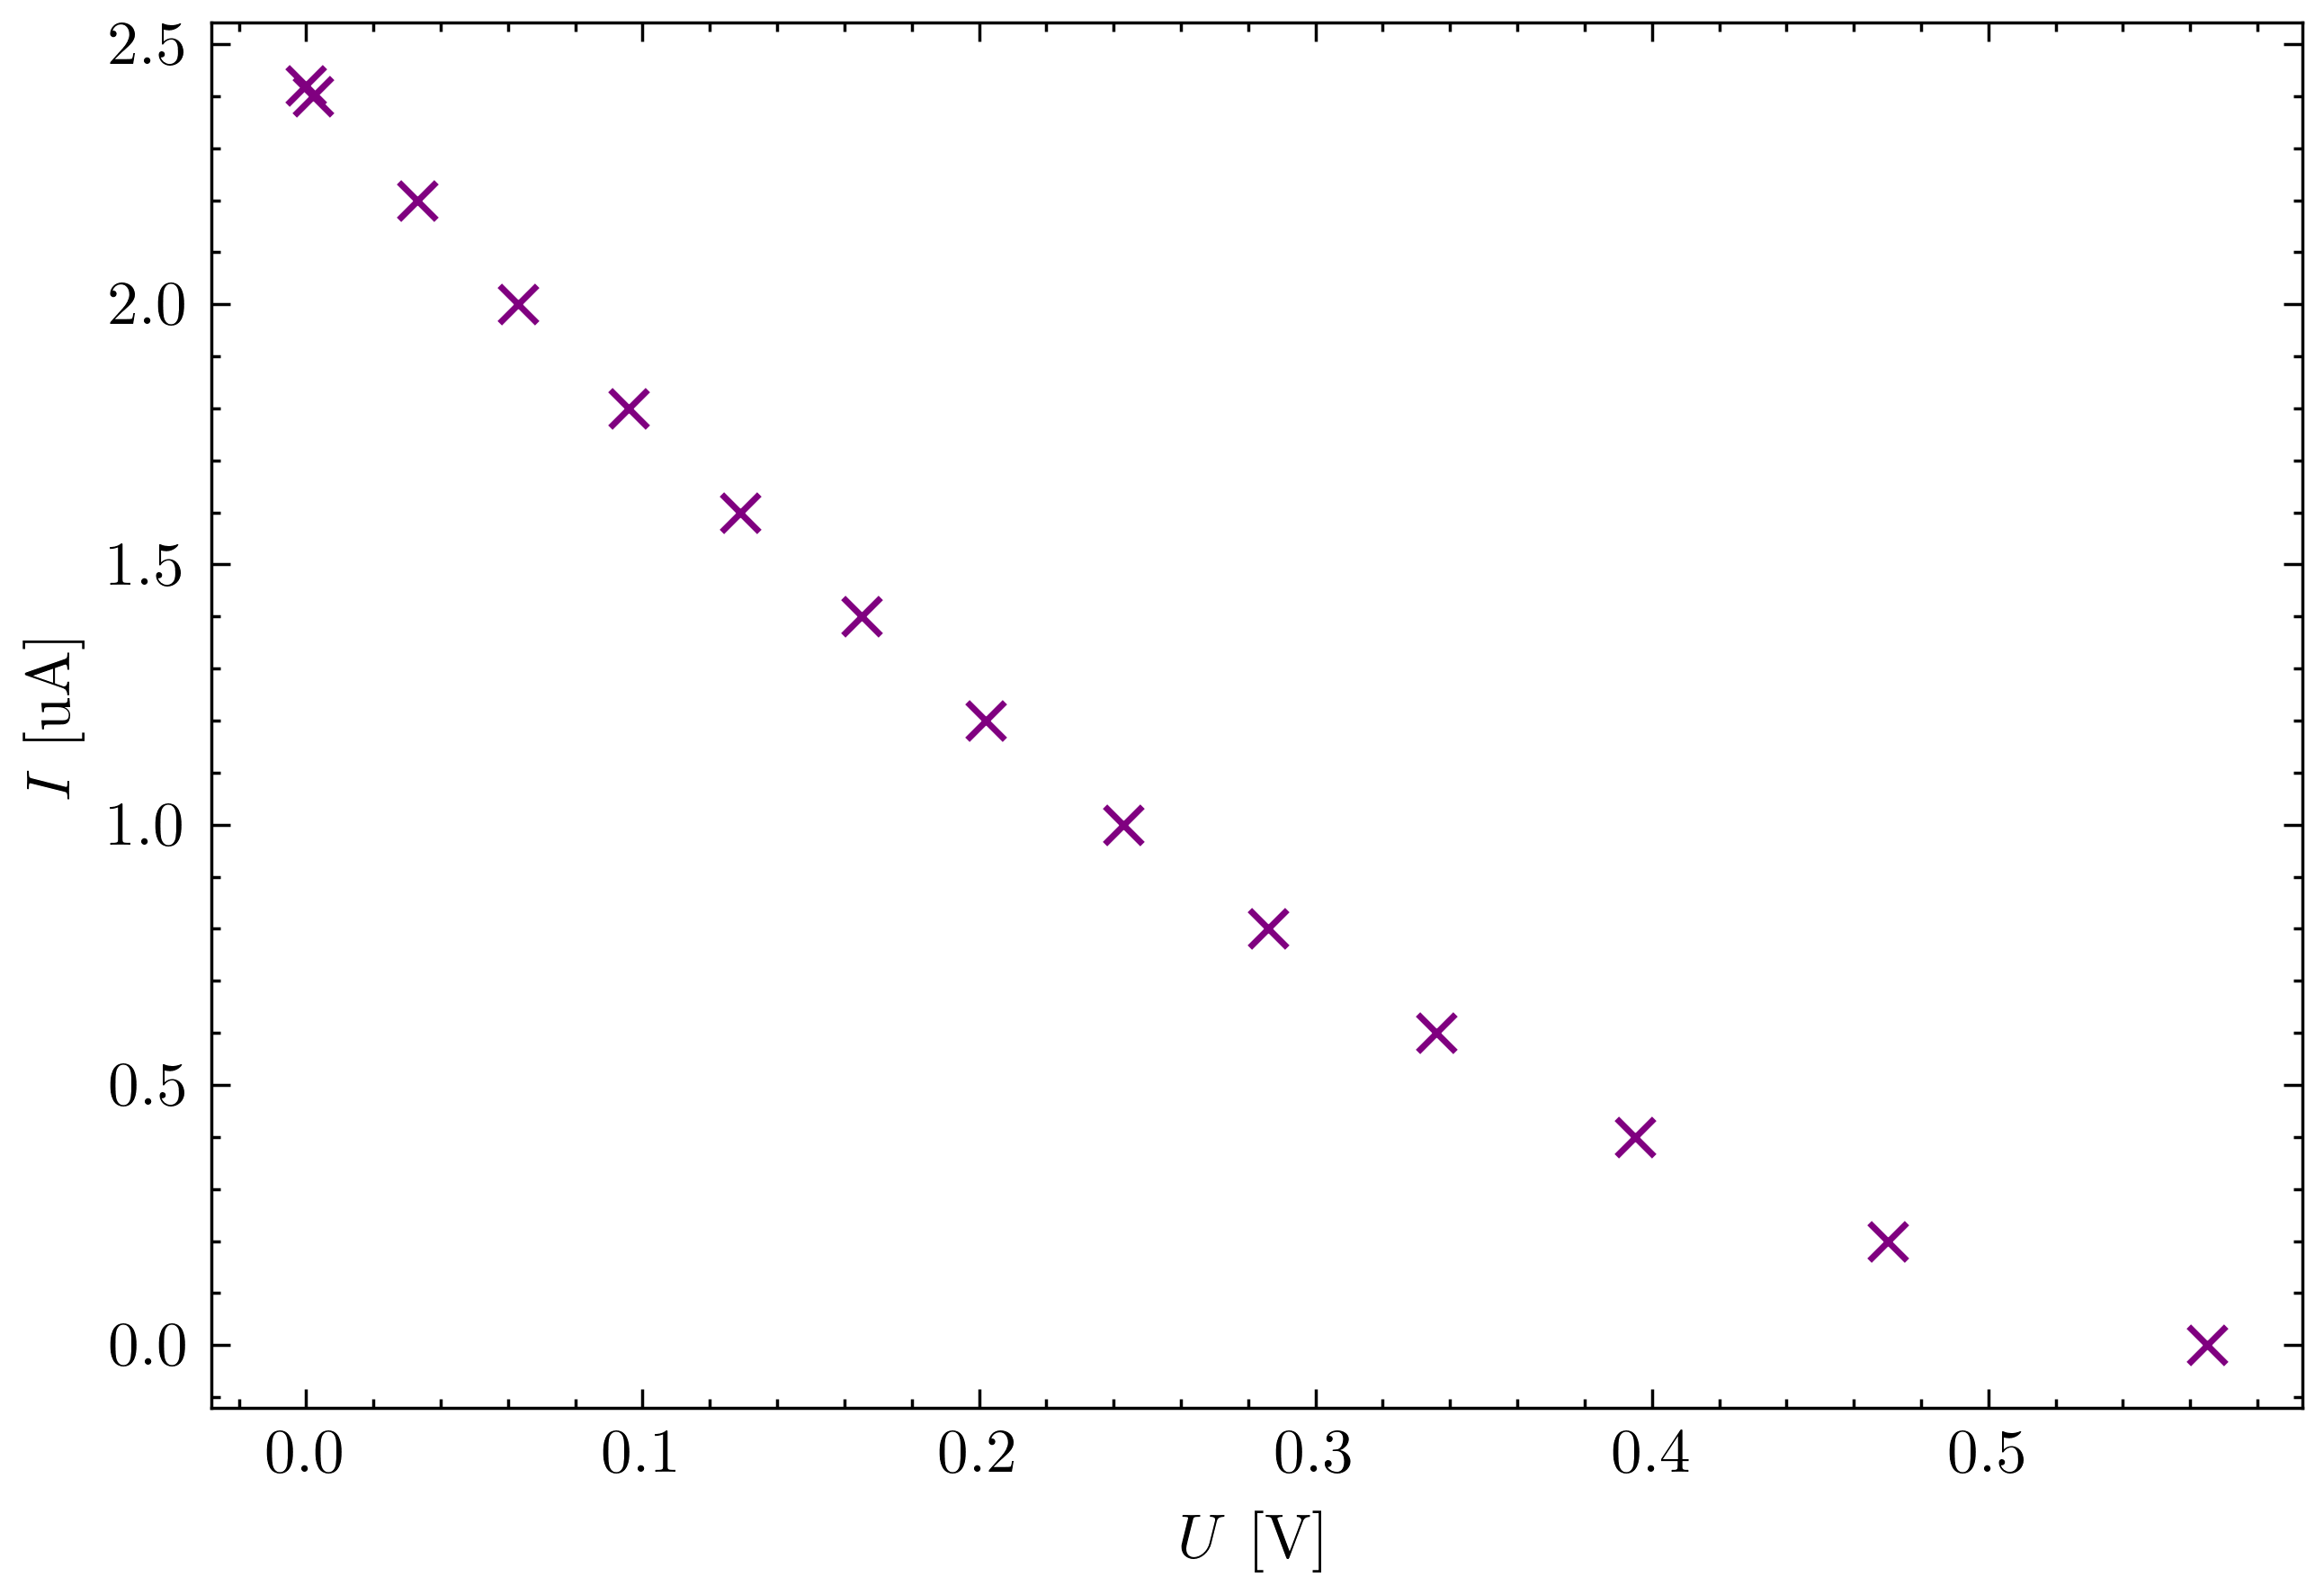
\includegraphics[width=0.75\linewidth]{purple.png}
    \caption{
    Zależność prądu fotokomórki $I$ od napięcia hamującego $U$
    dla koloru fioletowego.}
\end{figure}

\begin{figure}[H]
    \centering
    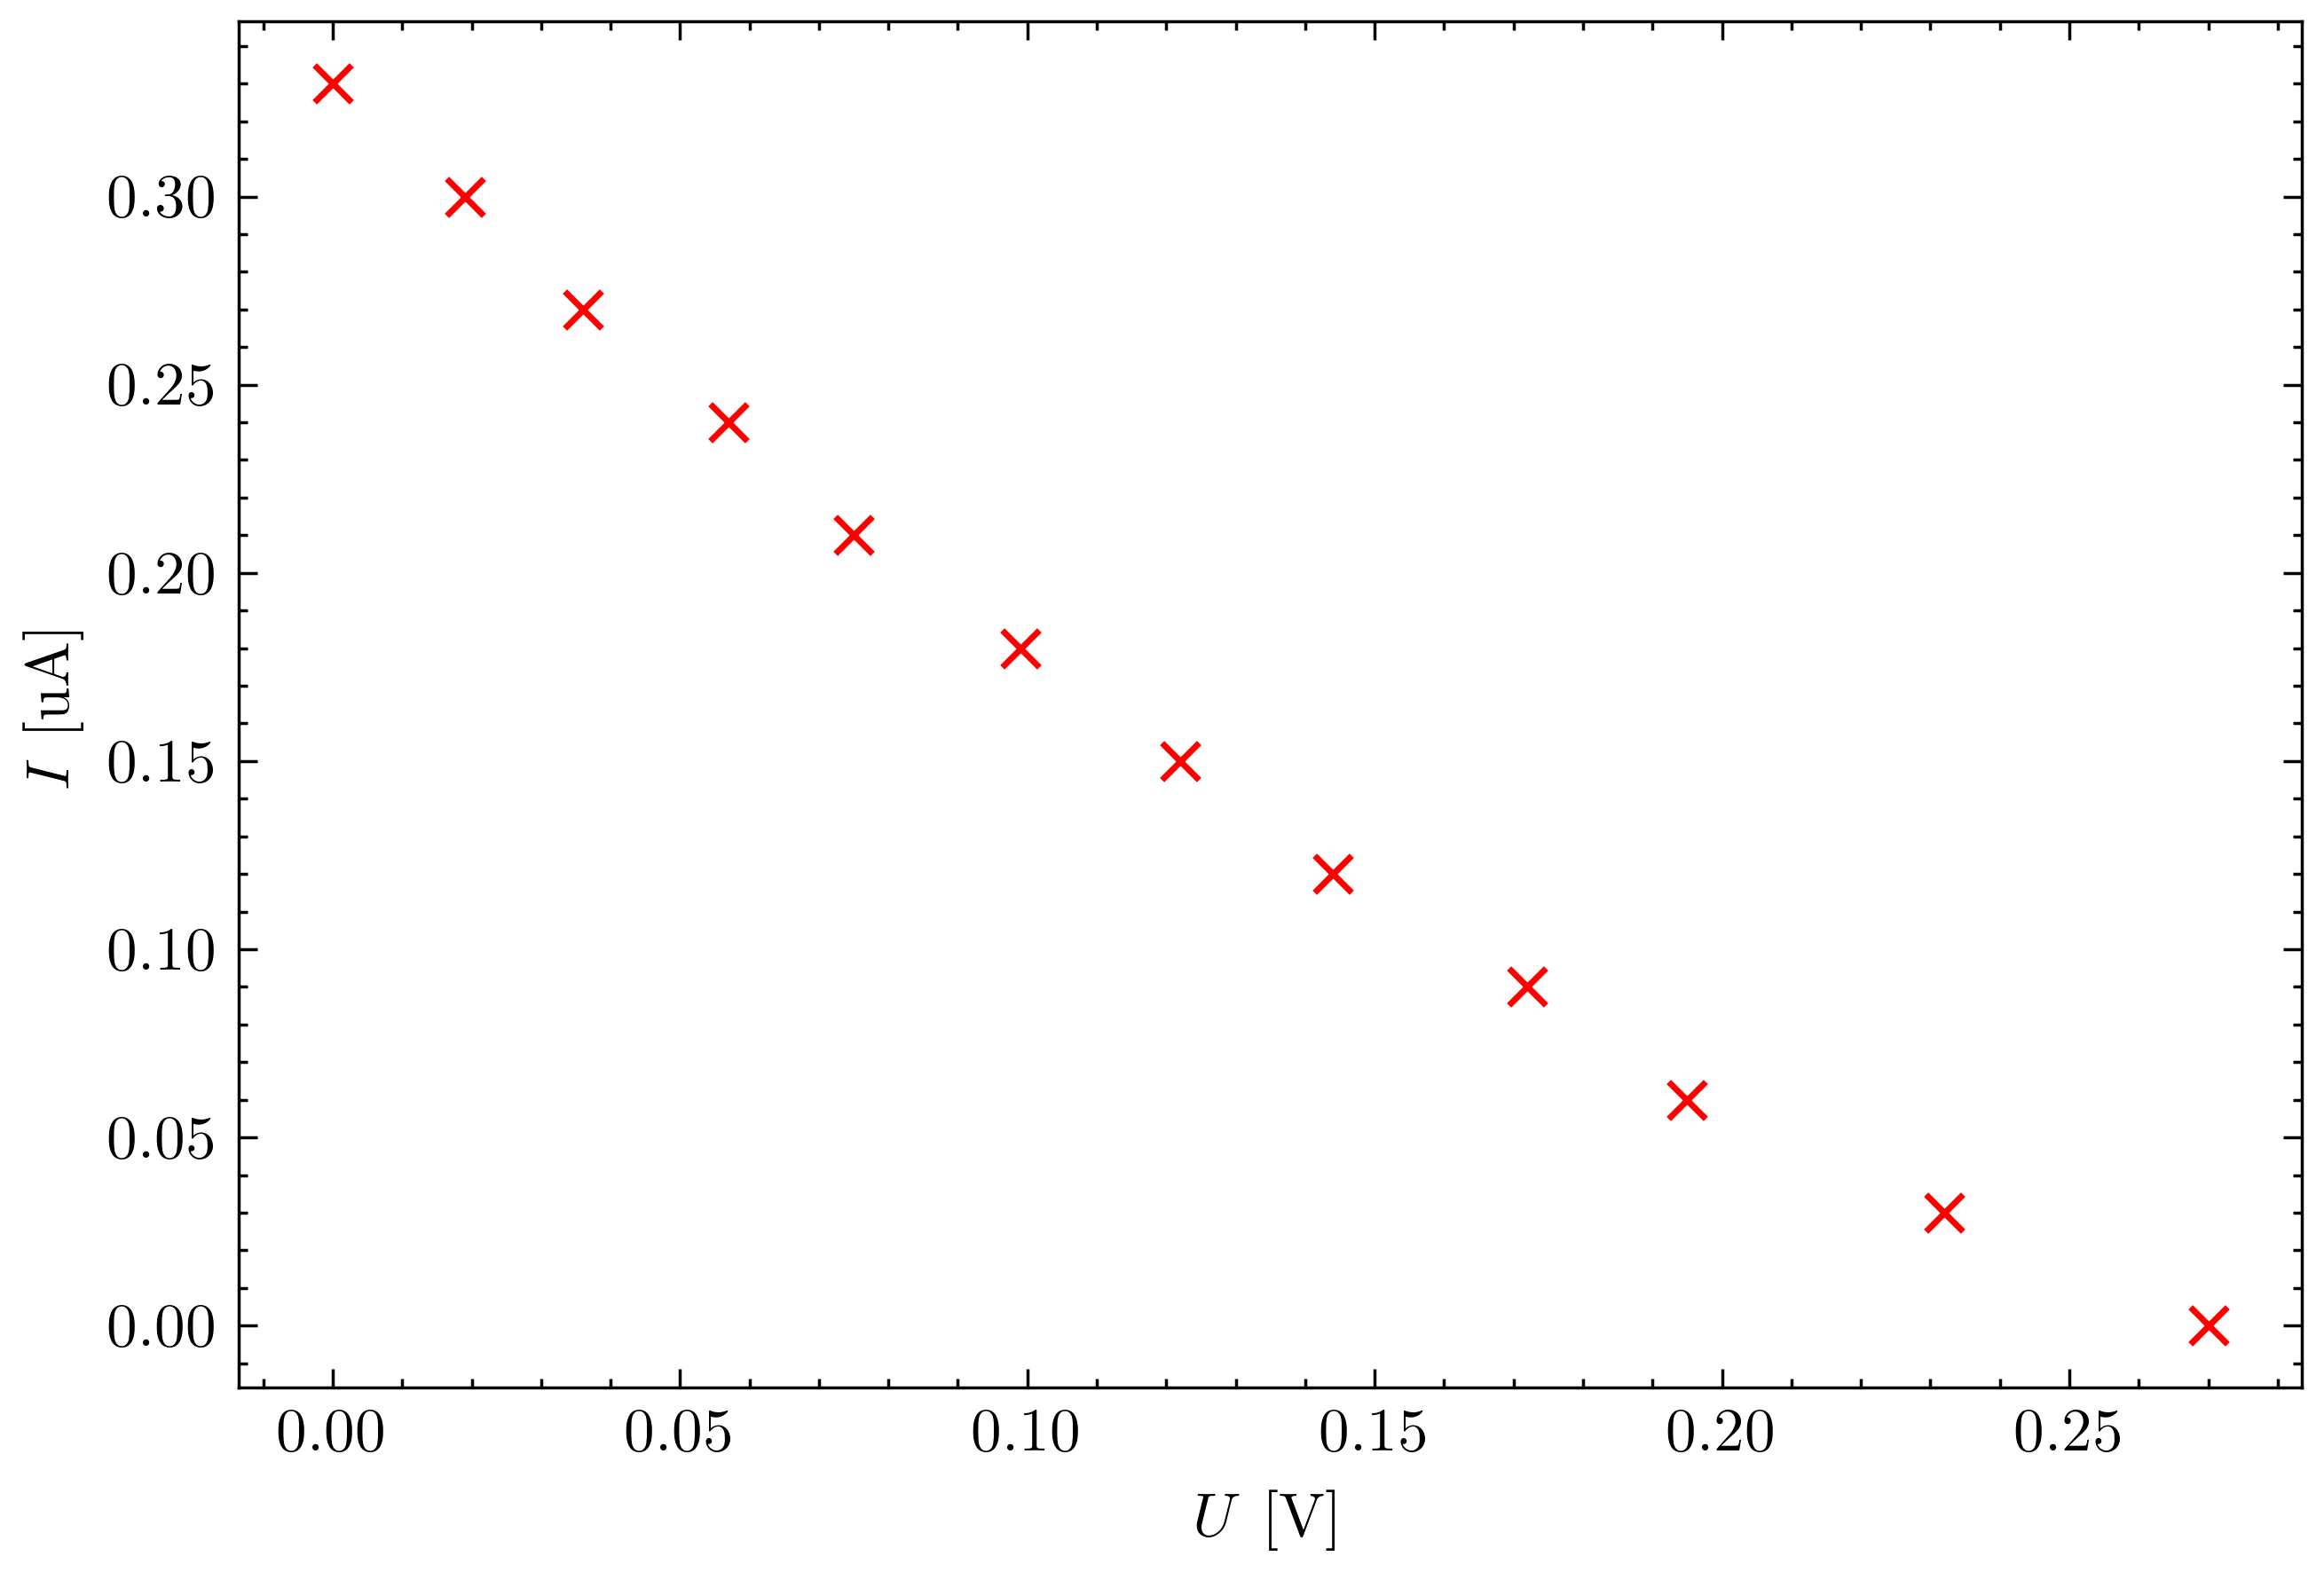
\includegraphics[width=0.75\linewidth]{red.png}
    \caption{
    Zależność prądu fotokomórki $I$ od napięcia hamującego $U$
    dla koloru czerwonego.}
\end{figure}


\begin{figure}[H]
    \centering
    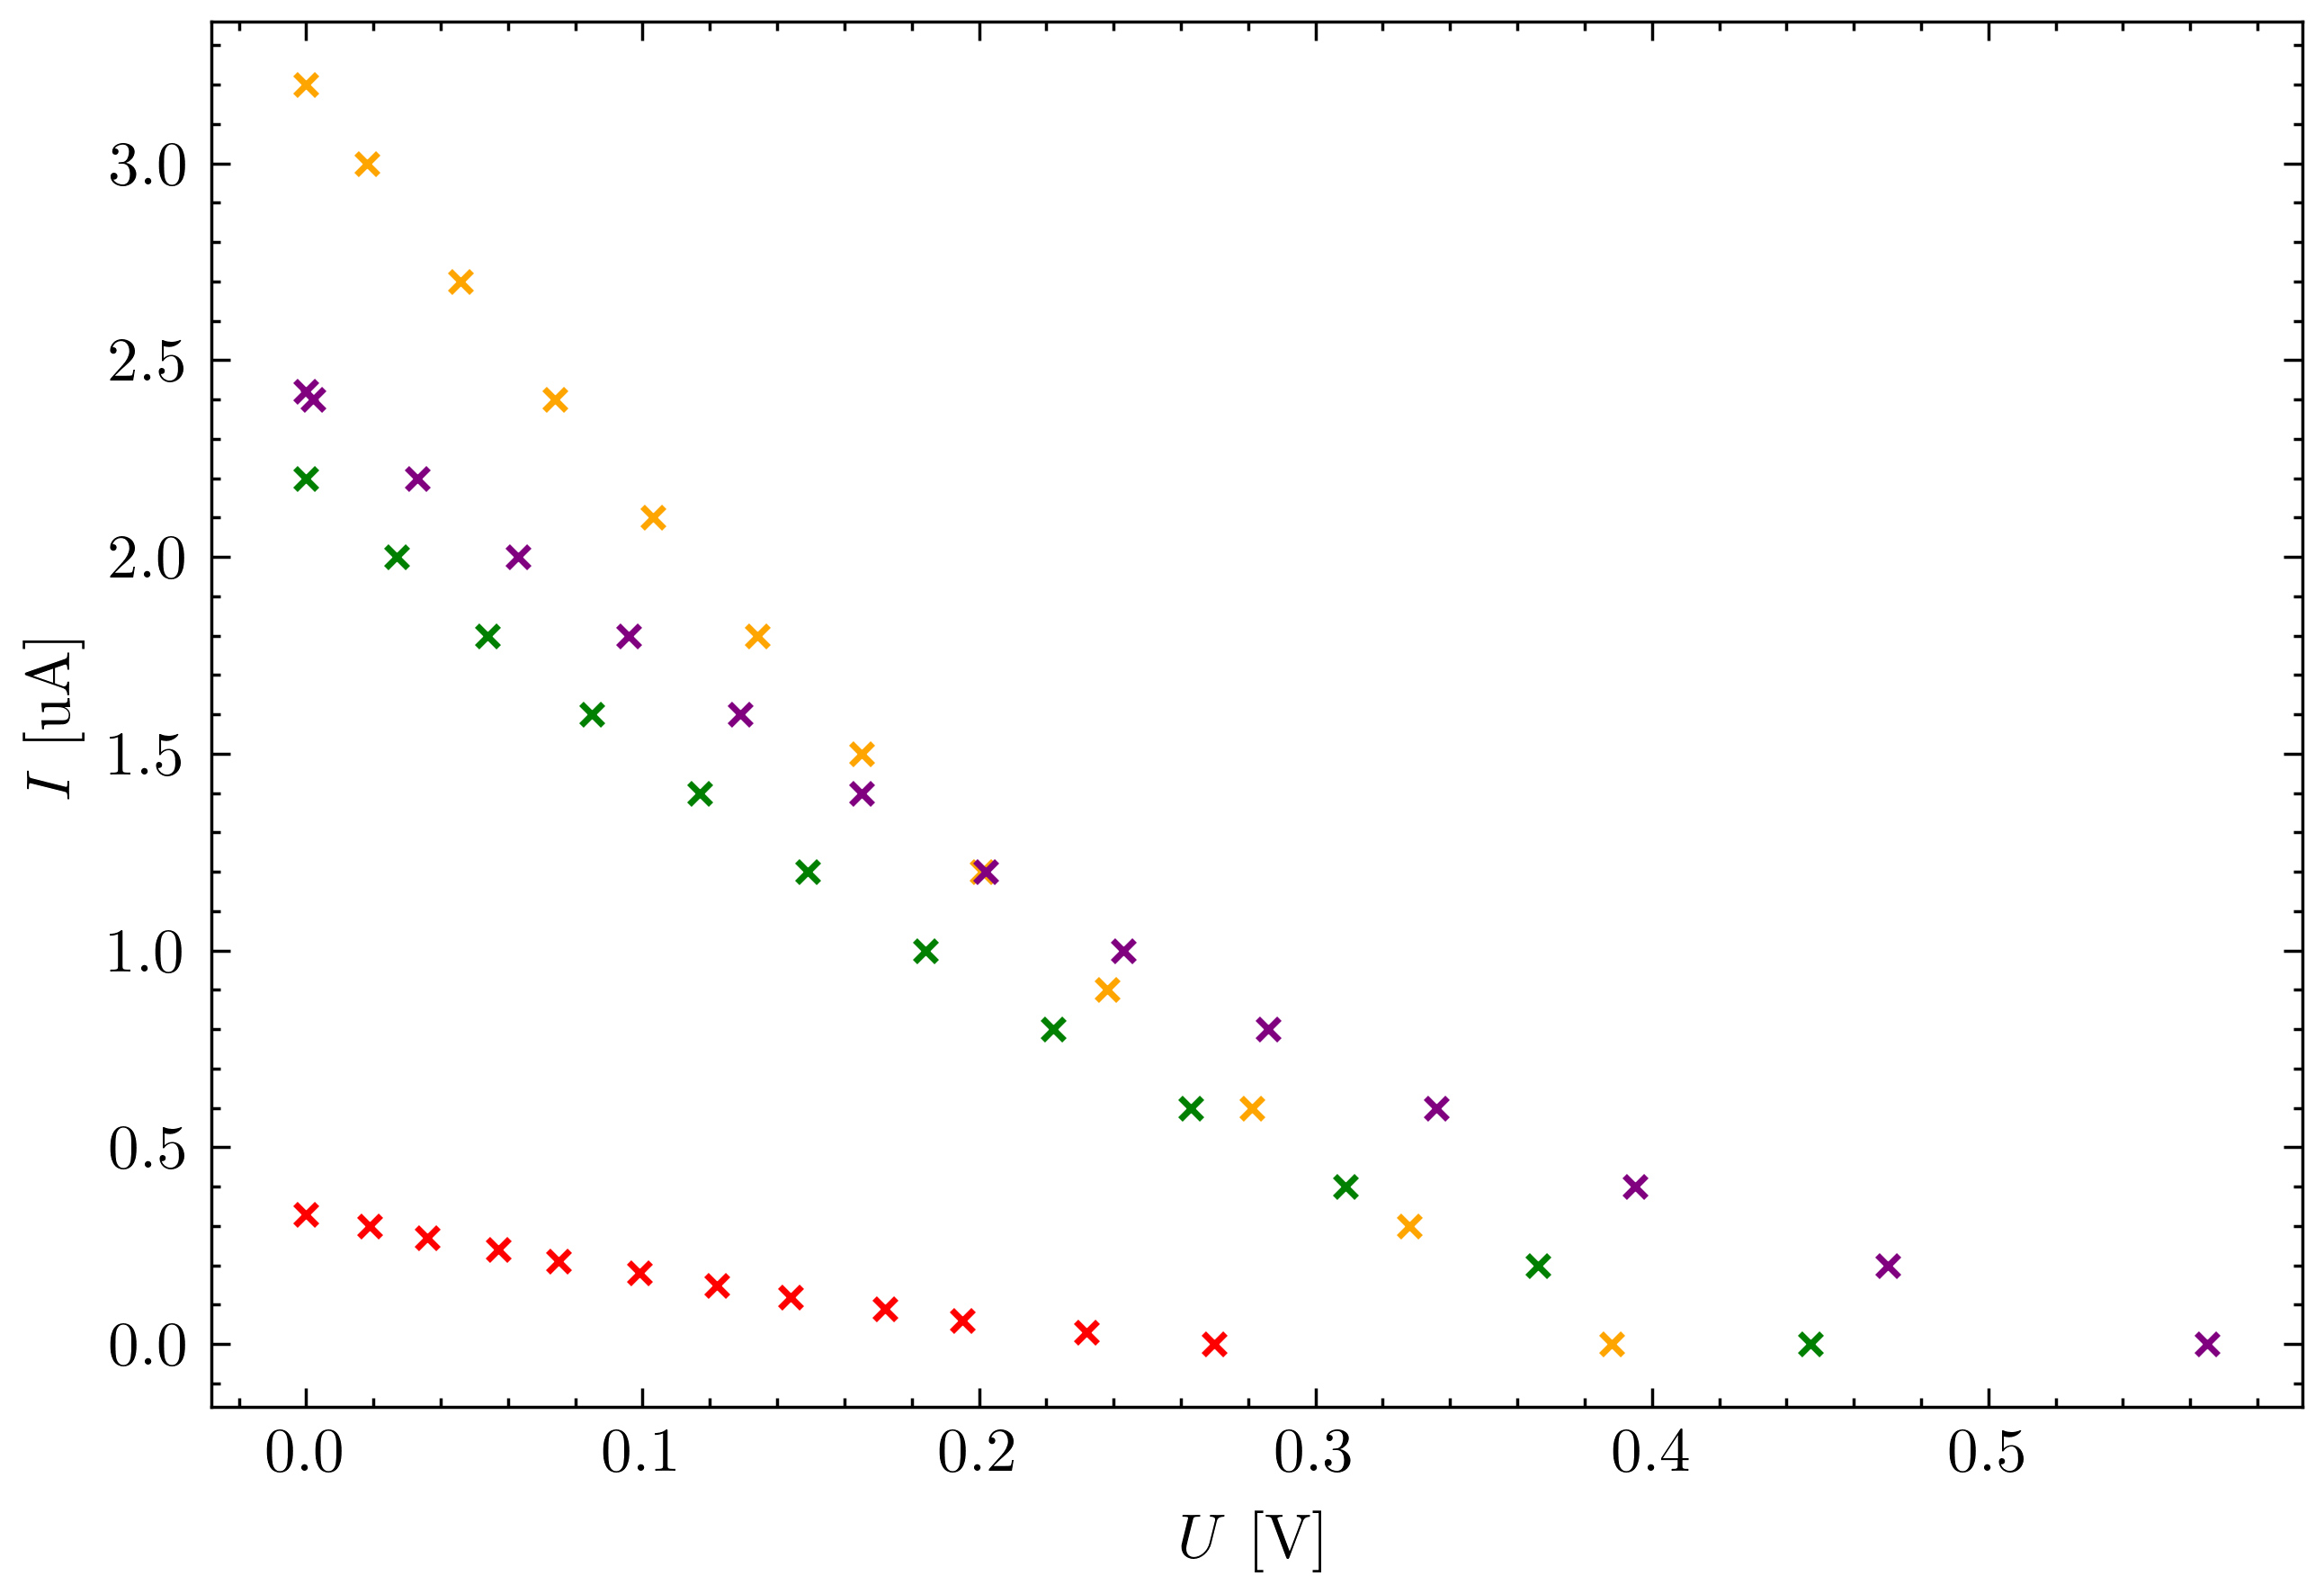
\includegraphics[width=0.75\linewidth]{allColors.png}
    \caption{Zbiorczy wykres zależności prądu fotokomórki $I$ od napięcia hamującego $U$
    dla wszystkich kolorów.
    }
\end{figure}

Jak widać wykresy $I(U)$ są
liniami prostymi, które
lekko się "wykrzywiają" gdy zbliżamy się do 
$I = 0$.

Ciekawy jest wykres zbiorczy dla wszystkich kolorów.
A w szczególności to co się dzieje z
kolorem żółtym. Prosta dla tego koloru
przecina prostą dla koloru zielonego oraz fioletowego,
co nie powinno się dziać.
Być może jest to spowodowane uszkodzeniem tego filtru,
lub nieumiejętnym lub niedokładnym włożeniem go
do kasety. Proste dla pozostałych kolorów zdają 
się być już zgodne z teorią.

\section{Wnioski}

\begin{enumerate}
    \item Wyliczona przez nas wartość stałej Plancka jest równa
    $h = 2.68 \cdot 10^{-34} \Js$
    jest ona bardzo zaniżona względnej wartości tabelarycznej.
    Jej niepewność $u(h)  = 0.72 \cdot 10^{-34} \Js$ jest bardzo 
    duża.
    Duży błąd oraz duża niepewność 
    najpewniej wynika z nieznanych nam 
    niedoskonałości urządzeń pomiarowych lub
    samych filtrów.
    \item Wyliczona przez nas praca wyjścia jest równa
    $W = 0.51 \volt$, jednakże wynik ten jest obarczony bardzo dużą 
    niepewnością pomiarową $u(W) = 0.25V$.
    \item Wykresy zależności prądu fotokomórki $I$ od 
    napięcia hamującego są liniami prostymi, 
    które jednak zatracają swój prosty
    kształt gdy zbliżamy napięcie zbliża się 
    do $U_h$.
    
    

    
\end{enumerate}
\end{document}
 
 
 

